\documentclass[a4paper,12pt,titlepage,twosided]{article}

\usepackage{amsmath}		% For math symbols
\usepackage{xcolor, graphicx}		% For including images

% for code segments
\usepackage{fancyvrb}	
\DefineVerbatimEnvironment{code}{Verbatim}{fontsize=\small}
\DefineVerbatimEnvironment{example}{Verbatim}{fontsize=\small}

\begin{document}

\title{Modelling/Geometric Transformations}

\author{Rajat Khanduja \\
	09010137 \\
	\and
	Bharat Khatri\\
	09010164}
\date{} %For empty date !

\maketitle

\tableofcontents
\pagebreak

\section{Modelling Transformations}
	Changes in orientation, size and shape are accomplished with Geometric transformations that alter the co-ordinate description of objects. The basic geometric transformations are :- \\
	\begin{itemize}
		\item Translation
		\item Scaling
		\item Rotation
		\item Reflection
		\item Shear
	\end{itemize}

	\subsection{OpenGL examples}
	In the text that follows, we use some OpenGL examples to illustrate how the transformations are performed using OpenGL functions. All transformations are being applied to a square of edge length 1 centred at (0,0), unless stated otherwise. 	
	\begin{figure}
		\centering
		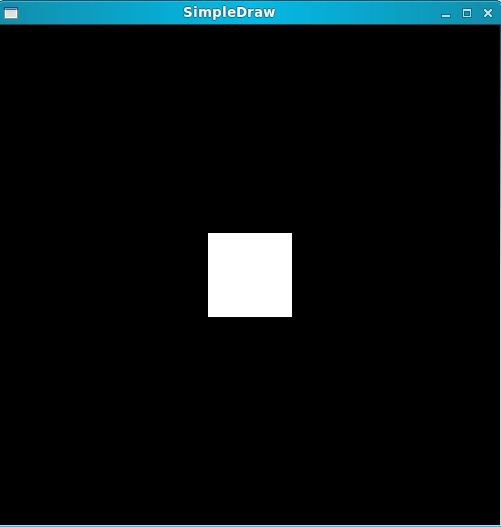
\includegraphics[height=80mm]{Images_final/Square.jpg}
		\caption{A square drawn using OpenGL.}
	\end{figure}
	\\
	Following is the part of the code to construct the square in discussion. 
	\begin{code}
		glPushMatrix ();
		glBegin (GL_POLYGON);
		glVertex2f (-0.5, -0.5);
		glVertex2f (-0.5, 0.5 );
		glVertex2f ( 0.5, 0.5 );
		glVertex2f ( 0.5, -0.5);
		glEnd ();
		glPopMatrix ();
	\end{code}
	
	In the discussions that follow, only the transformation code is provided which has to be used before plotting the vertices (\emph{glVertex2f}) but after pushing the matrix using \emph{glPushMatrix}

\pagebreak
\section{Translation}
	\subsection{Introduction}
	A \emph{translation} is applied to an object by repositioning it along a straight line path from one coordinate location to another. Mathematically, translation is achieved by adding the translation distance, $t_x$ and $t_y$, to the original coordinate position $(x,y)$ to move to the new position $(x^{'},y^{'})$.
	\begin{equation*}
		x^{'} = x + t_x
	\end{equation*}
	\begin{equation*}
		y^{'} = y + t_y
	\end{equation*}
	Translation can be achieved by the following transformation :-\\
	\\
	For 2D translation :-
	\begin {equation*}
		\begin{bmatrix}
			1 & 0 & 0 & t_x \\
			0 & 1 & 0 & t_y \\
			0 & 0 & 1 & 0 \\
			0 & 0 & 0 & 1
		\end{bmatrix}
	\end{equation*}
	\\
	For 3D translation :-
	\begin {equation}
		\begin{bmatrix}
			1 & 0 & 0 & t_x \\
			0 & 1 & 0 & t_y \\
			0 & 0 & 1 & t_z \\
			0 & 0 & 0 & 1
			\label{translation_eq}
		\end{bmatrix}
	\end{equation}
%\begin {equation*}
%	\begin{bmatrix}
		
	\subsection{Translation in OpenGL}
		\begin{figure}
			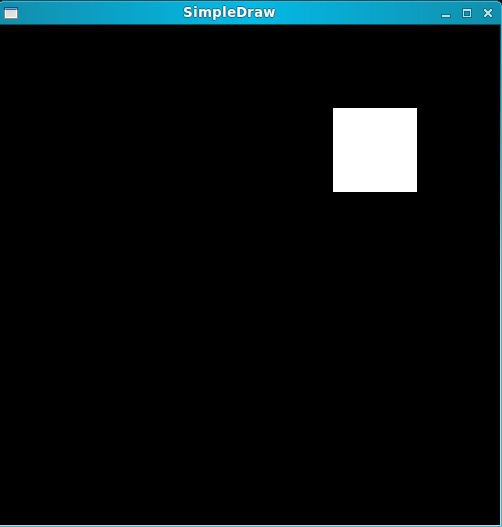
\includegraphics[height=80mm]{Images_final/Translated_square.jpg}
			\label{fig:translated}
			\caption{Translated square}
		\end{figure}
		Translation can be achieved in OpenGL using the function \emph{glTranslate}. \\ \\
		The same could be achieved using the transformation matrix described in \eqref{translation_eq}.
		\begin{code}
			// Column major matrix.
			GLdouble t_x = 1;
			GLdouble t_y = 1;
			GLdouble t_z = 0;
			GLdouble translation_matrix[] = { 1, 0, 0, 0,
							  0, 1, 0, 0,
							  0, 0, 1, 0,
							  t_x, t_y, t_z, 1};	

			glMultMatrix (translation_matrix);
		\end{code}
		The effect of the same can be seen in Figure ~\ref{fig:translated}.
	
		
\pagebreak
\pagebreak
\section{Scaling}
\emph{Scaling} a coordinate means multiplying each of its components by a scalar. 


\begin {equation*}
	\begin{bmatrix}
		c & 0 & 0 & 0 \\
		0 & c & 0 & 0 \\
		0 & 0 & c & 0 \\
		0 & 0 & 0 & 1
	\end{bmatrix}
\end{equation*}

\pagebreak
\section{2D Rotation}
A \emph{2D Rotation} is applied to an object by repositioning it along a circular path in any of the three x-y, y-z or z-x planes.

\pagebreak
\section{Reflection}
A \emph{reflection} is a transformation that produces the mirror image of an object relative to an axis of reflection by rotating the object $180^\circ$ about the reflection axis. 
\pagebreak
\section{Shear}
A \emph{transformation} that distorts the shape of an object such that the transformed shape appears as if the object were composed of internal layers that had been caused to slide over each other.

\pagebreak
\end{document}
